\procTitle{Перспективные методы биологической рекультивации на отвалах Якутии}
\procTitleNewLine{Перспективные методы биологической рекультивации\\на отвалах Якутии}

\procAuthor{Никифоров~А.\,А., Миронова~С.\,И., Гаврильева~Л.\,Д.}
\procEmail{aloooosha1991@mail.ru, mironova47@mail.ru, adoxa@mail.ru}
\procOrganization{НИИПЭС СВФУ} \procCity{Якутск}


\index{n@Никифоров~А.\,А.}
\index{m@Миронова~С.\,И.}
\index{g@Гаврильева~Л.\,Д.}

\makeProcTitleNewLine

Нарушение земель происходит при разработке месторождений полезных ископаемых, прокладке трубопроводов, проведении строительных, мелиоративных, лесозаготовительных,\;\;геологоразведочных,\;\;испытательных,\;\;эксплуатационных,\;\;проектно-изыскательных\\и~иных работ, поэтому на Севере нашей страны актуальны вопросы их восстановления с~применением наиболее эффективных и экономически целесообразных способов. Практическое применение на территории Республики Саха (Якутия) на нарушенных землях предприятий, занимающихся алмазо- и угледобычей, на россыпных месторождениях золота находятся только на опытно-экспериментальных стадиях и имеют только рекомендательный характер.  Применение старики (ветоши) для биологической рекультивации на отвалах пустых пород карьера <<Айхал>> проведено впервые на нарушенных территориях Крайнего Севера. Старика (ветошь)~--- сухая прошлогодняя трава на лугах, опавшие листья. В~её~состав входят все нескошенные растения или отава после сенокошения, т.\,е. это луговые злаки, бобовые и разнотравье, а также (реже) осоковые растения.

\textbf{Целью} работы является поиск наиболее эффективных способов для восстановления нарушенных земель добывающих предприятий.

\textbf{В задачи} работы входила оценка основных факторов, воздействующих на зарастание отвалов растительностью, проведение опытно-экс\-пе\-ри\-мен\-таль\-ных работ с применением нетрадиционного материала, оценка эффективности способа, рассмотрение возможности внедрения способа в промышленных масштабах.

\textbf{Материал и методы исследования}

Первые опытные работы по биологической рекультивации на отвалах алмазодобывающей промышленности в республике были проведены сотрудниками института <<Якутнипроалмаз>> на участке площадью 2\,га, отсыпанном плодородным слоем разной мощности, испытаны 19 видов многолетних трав [2].

С развитием промышленных предприятий резко увеличились территории нарушенных земель, у которых в первую очередь разрушается почвенно-растительный покров, а во вторую запускается цепочка эрозионных процессов. На нарушенных территориях образуются хвостохранилища, отвалы пустых пород, карьеры и др. [1].

Начиная с 2010\,г. институтом прикладной экологии Севера СВФУ проведены опытно-экспериментальные работы на отвалах пустых пород карьера <<Айхал>> и в 2018\,г. на отвалах угольного разреза <<Кангаласский>> с применением нетрадиционных материалов. При рекогносцировочном исследовании поверхности отвала выбрали наиболее ровную поверхность и откосы с наименьшим углом (45\dg), высота отвала 60--70 м (рис. 1).

При заложении площадки очистили от крупных валунов и глыб, размер площадки 20\,$\times$\,20\,м, на откосе 10\,$\times$\,10\,м. Вначале на опытно-экс\-пе\-ри\-мен\-таль\-ной площадке проведён посев семян из расчёта 30\,кг/га и внесение минеральных удобрений (<<Азофоска>>) из расчёта 100\,кг/га действующего вещества. Сверху площадка была накрыта старикой, закреплена тонким слоем песка и камнями (рис. 2).

Геоботаническое описание опытно-экспериментальной площадки проводилось с учётом общего проективного покрытия в процентах, средней высоты, видового состава, проективного покрытия с применением шкалы Б.\,М.\,Миркина [3].

Сбор старики проводился по долине р.\,Сохсолох с помощью косилок, вил и других ручных инструментов. Для угольного разреза <<Кангаласский>> был применён прошлогодний рулон сена, который вполне подходит для проведения опытно-экспериментальных работ.

\textbf{Результаты исследований и их обсуждение}

На опытно-экспериментальной площадке в отвале пустых пород карьера <<Айхал>> среднее проективное покрытие травостоя в первый год составило 40\,\%, на второй год~--- 50\,\%, а~максимального значения достигло 80\,\%, средняя высота травостоя в первый год 3\,см, а~на~второй год~--- 45\,см. Видовой состав в первый год (2011\,г.) составлял в количестве от 1--2, в последующие годы увеличился до 7\,видов (рис. 3).

\begin{figure}
  \begin{center}
    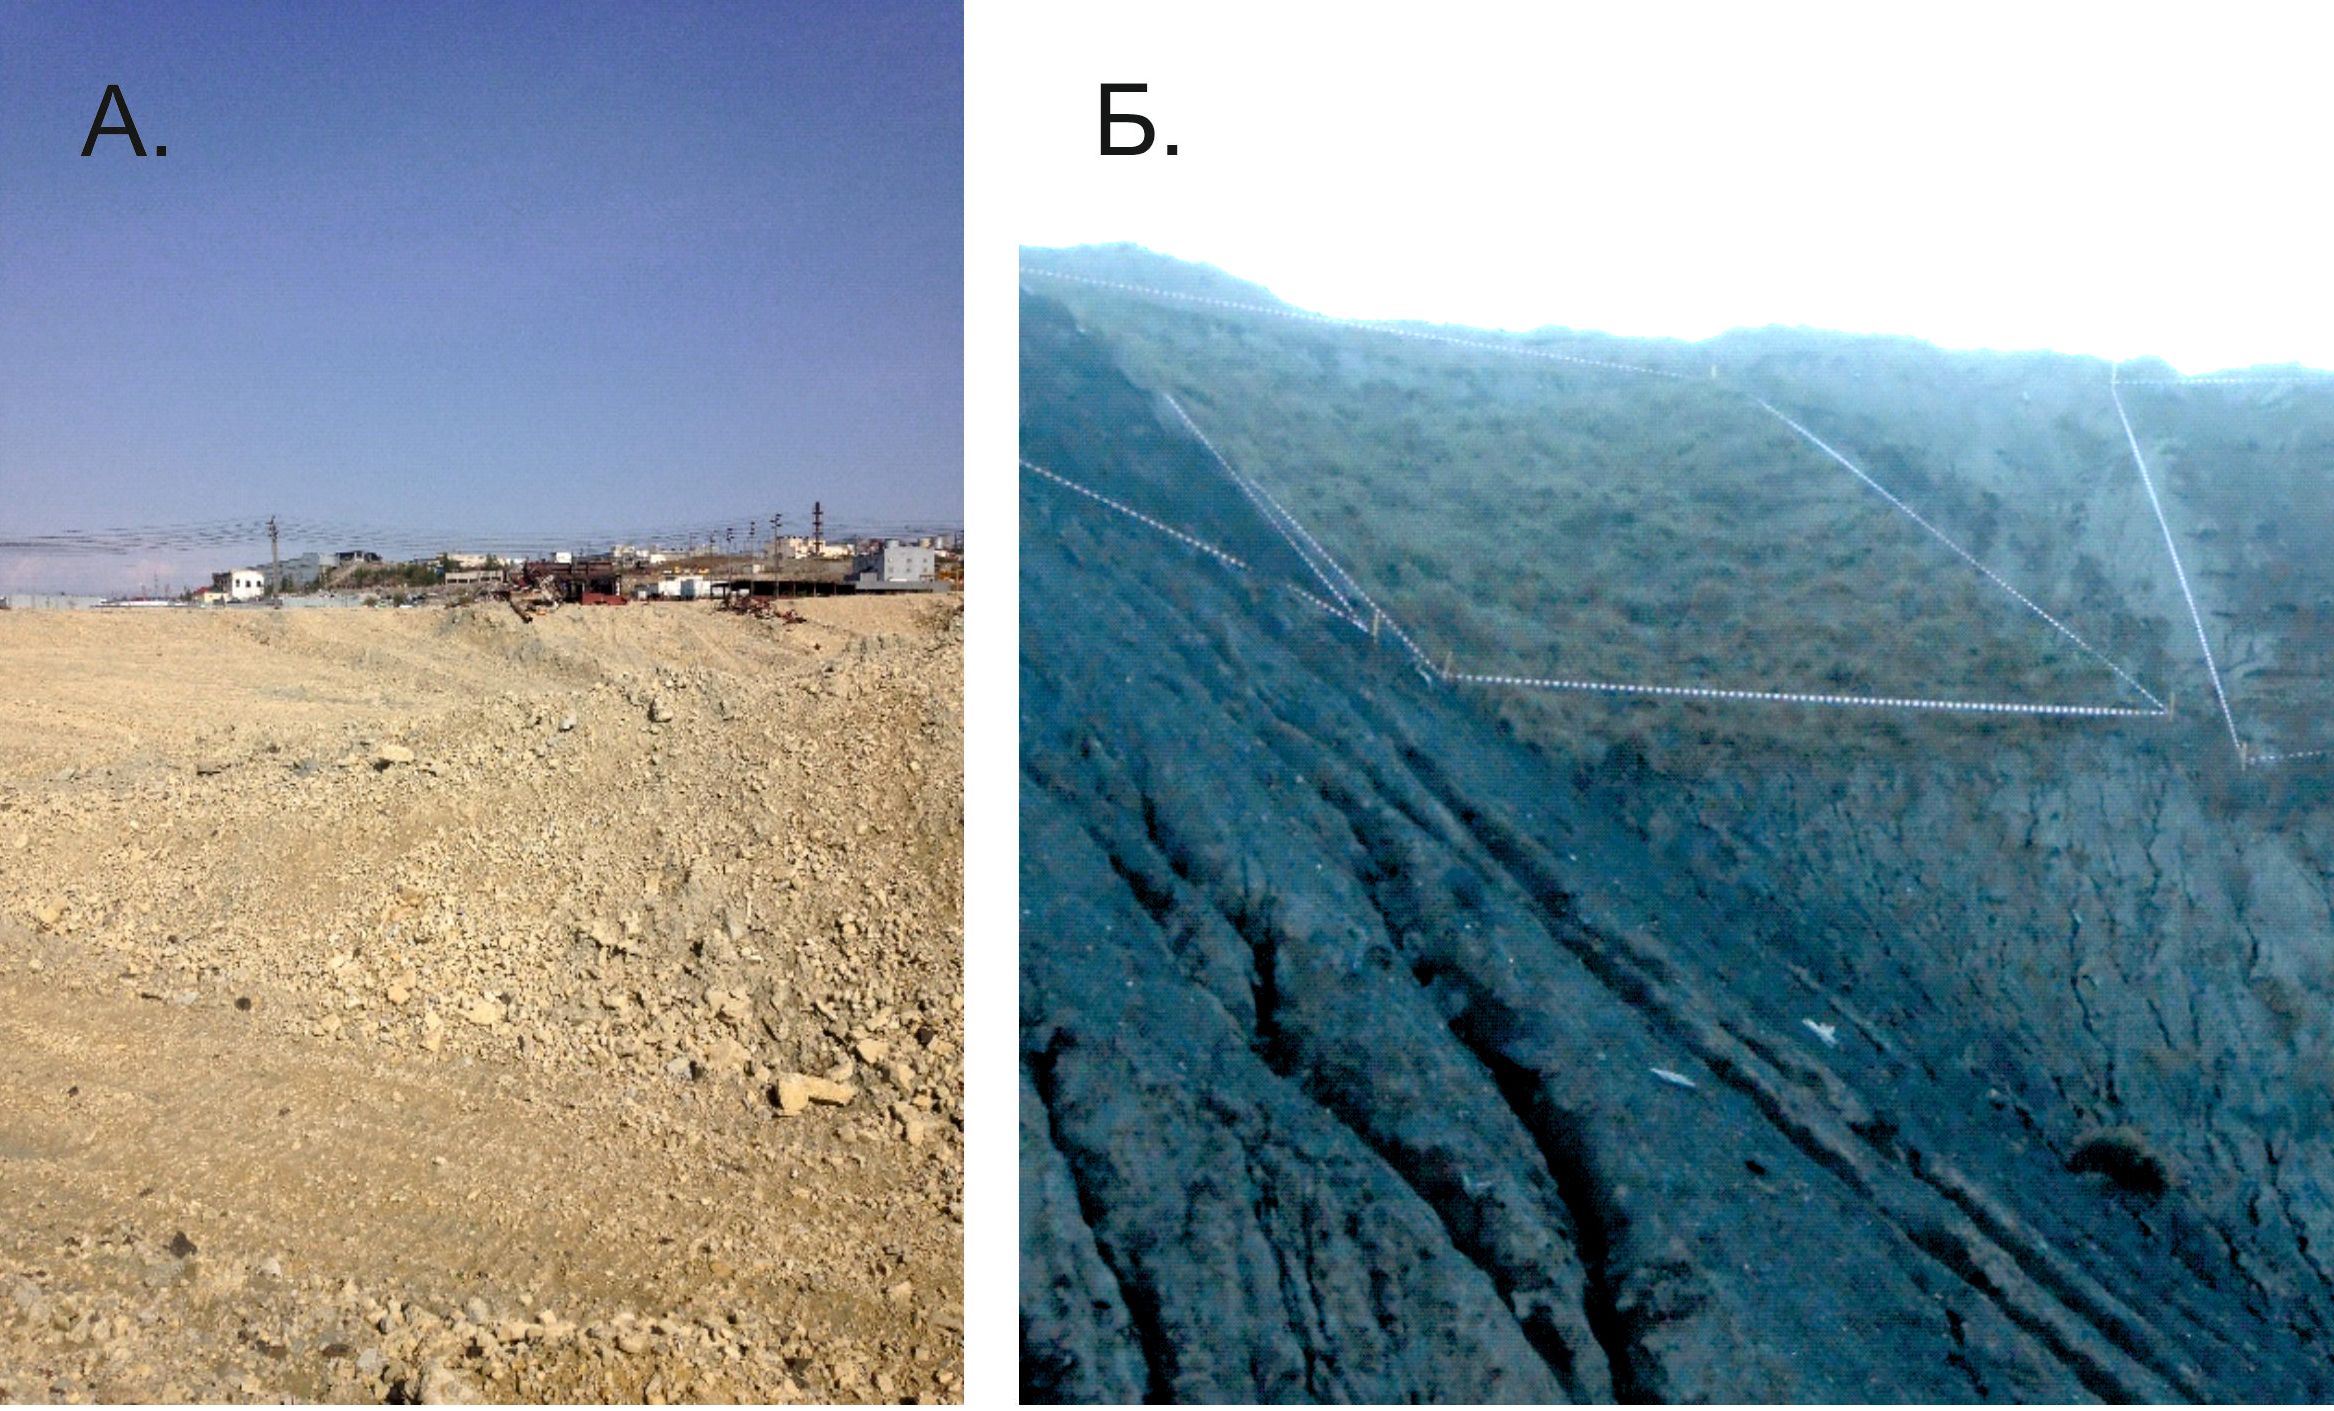
\includegraphics[width=0.9\textwidth]{authors/nekiforov-fig1.jpg}
  \end{center}
  \caption{Поверхность отвала пустых пород карьера <<Айхал>> (А) и откос отвала угольного разреза <<Кангаласский>> (Б)}
  \label{fig:nekiforov-fig1}
\end{figure}

\begin{figure}
  \begin{center}
    
\includegraphics[width=0.9\textwidth]{authors/nekiforov-fig2.jpg}
  \end{center}
  \caption{Опытно-экспериментальная площадка, накрытая старикой:
  А~--- отвал пустых пород карьера <<Айхал>>; Б~-- отвал угольного разреза <<Кангаласский>>}
  \label{fig:nekiforov-fig2}
\end{figure}

\begin{figure}
  \begin{center}
    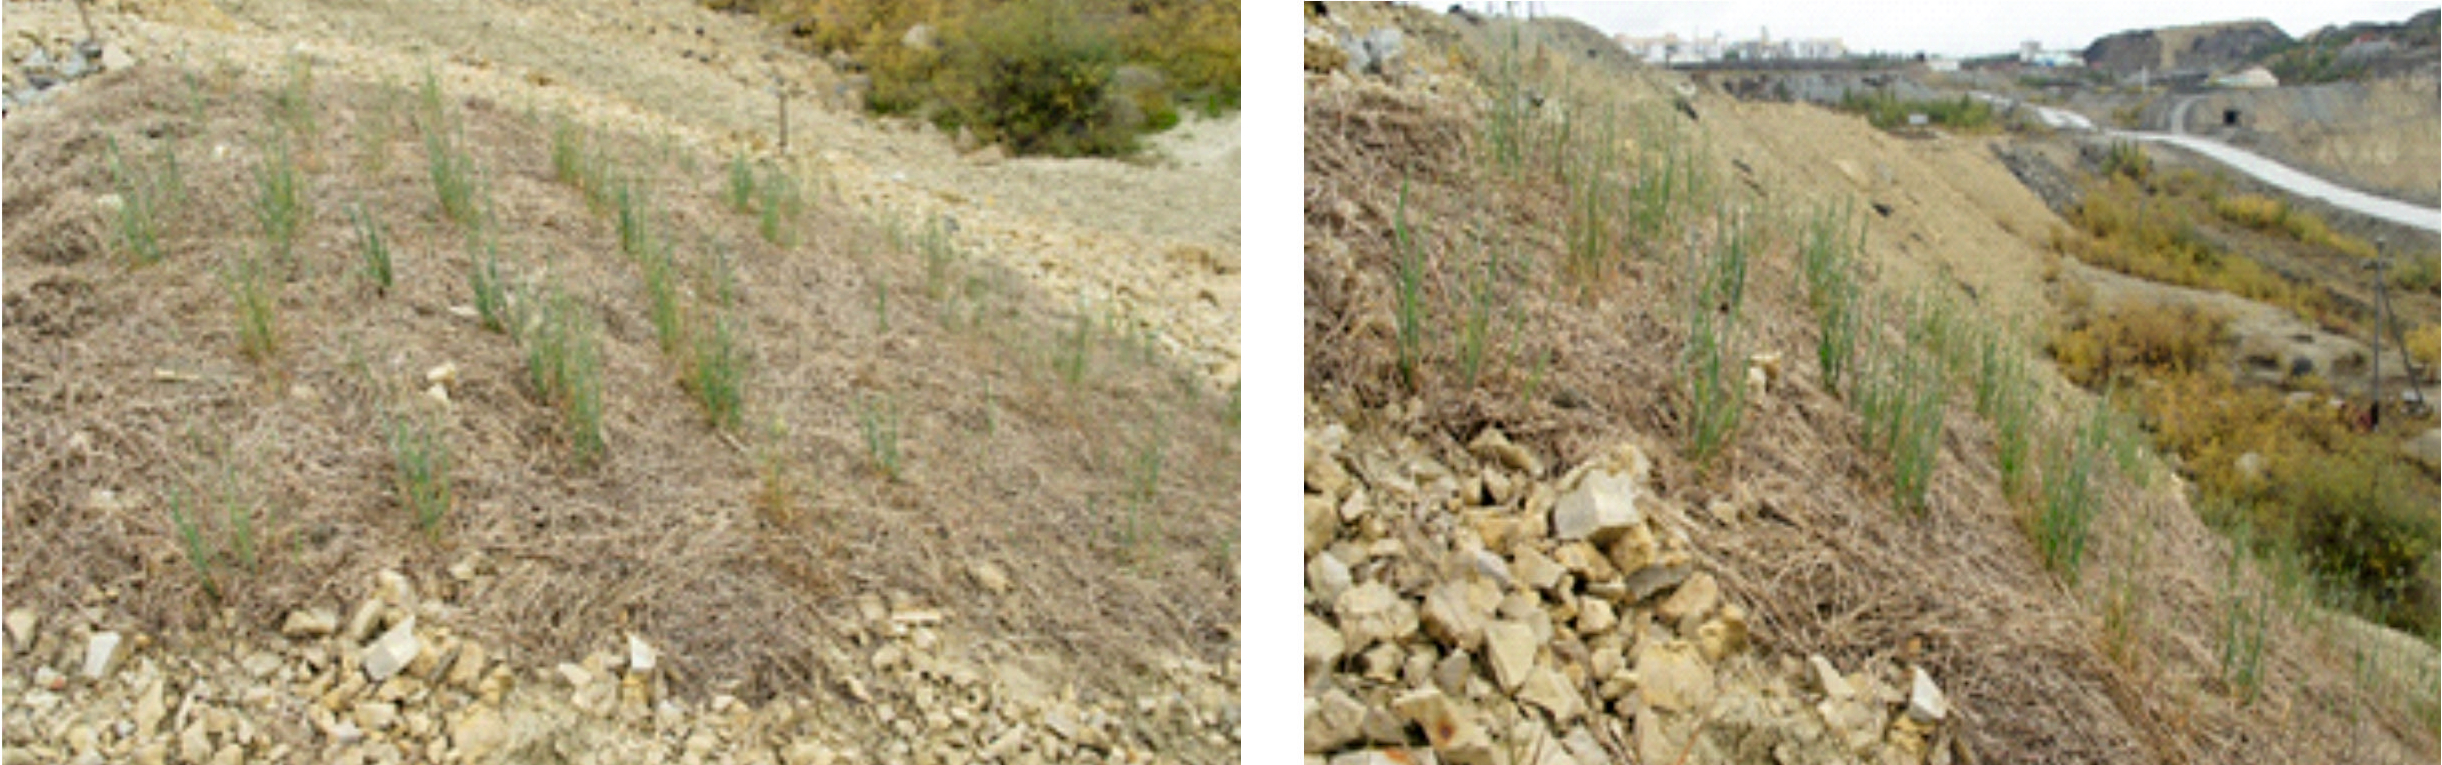
\includegraphics[width=0.9\textwidth]{authors/nekiforov-fig3.jpg}
  \end{center}
  \caption{Опытно-экспериментальная площадка с применением старики (ветоши) на отвале пустых пород карьера <<Айхал>>}
  \label{fig:nekiforov-fig3}
\end{figure}


На опытно-экспериментальной площадке в отвале угольного разреза <<Кангаласский>> среднее проективное покрытие травостоя на май составило 40--50\,\%, средняя высота 10--15\,см (май), видны всходы злаков и разнотравья. При наблюдении в~июне общее проективное покрытие составило 50--60\,\%, всхожесть высеянных трав составила 80\,\%, видовой состав насчитывал до 7 видов (рис. 4).

\begin{figure}
  \begin{center}
    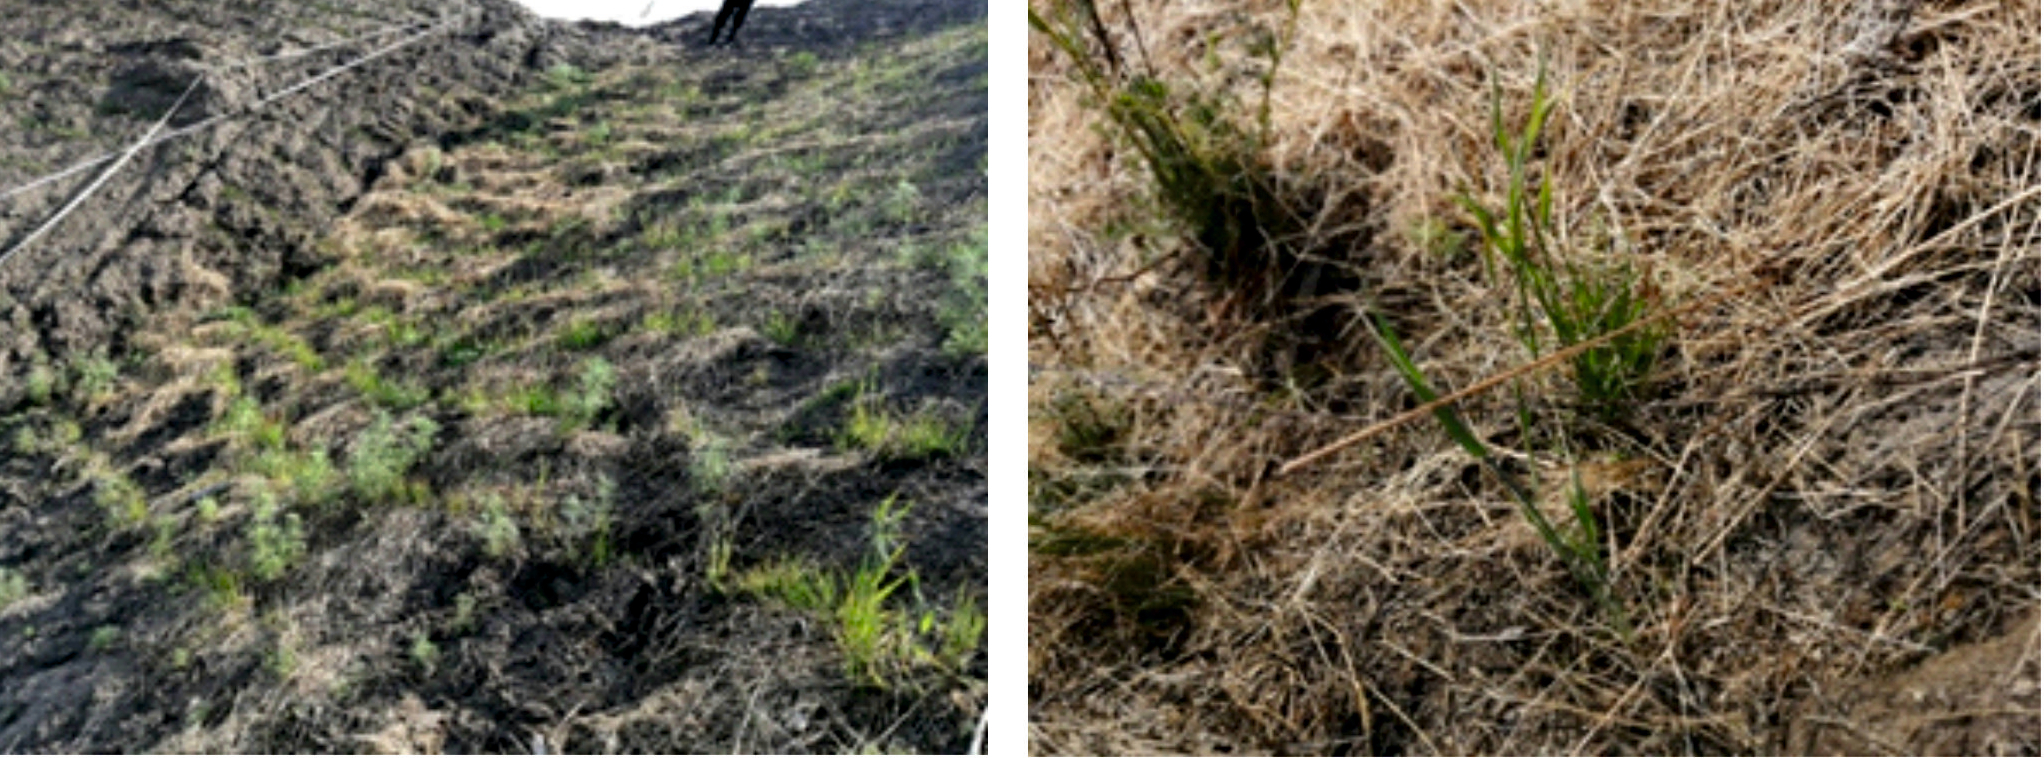
\includegraphics[width=0.9\textwidth]{authors/nekiforov-fig4.jpg}
  \end{center}
  \caption{Опытно-экспериментальная площадка с применением старики (ветоши) на отвале угольного разреза <<Кангаласский>>}
  \label{fig:nekiforov-fig4}
\end{figure}


Способ показал с перспективной стороны для внедрения в промышленных масштабах с учётом разработки технологий сбора и применения на более больших территориях. Применение старики в биологической рекультивации отвалов алмазодобычи в республике проведено впервые. В других странах этот метод применяют для других целей и в небольших объёмах только для огородов, теплиц, чаще всего в частном секторе. К применению нетрадиционного способа подтолкнули именно условия нашего региона~--- это суровый климат, экономическая целесообразность, отсутствие на данной территории потенциально плодородного слоя для отсыпки отвалов.
\clearpage
В других регионах России и мира отсыпка потенциально плодородным слоем нарушенных земель при биологической рекультивации обязательна. В нашей ситуации отсыпка плодородного слоя фактически невозможна из-за его отсутствия или экономической нецелесообразности отсыпки, учитывая характер подстилающих пород траппового характера.

\textbf{Выводы}

В результате опытно-экспериментальных работ по биологической рекультивации отвалов карьера <<Айхал>> и отвалов угольного разреза <<Кангаласский>> способ применения старики показал наиболее эффективные результаты.

В последующем можно повсеместно применять укрывной материал без привязки к сезонным изменениям. В отсутствие регулярного полива старика может послужить для задержания влаги и защитным слоем для всхожести семян, а при разложении~--- питательным субстратом для роста и питания растений.

\begin{thebibliography}{99}


\bibitem{}
ГОСТ Р 57446-2017. Наилучшие доступные технологии. Рекультивация нарушенных земель и~земельных участков. Восстановление биологического разнообразия (с Поправкой).~--- М.~: Стандартинформ, 2019.~--- 47\,с.


\bibitem{}
\BibAuthor{Лебедева\,H.\,A., Лонкунова\,А.\,Я.} Биологическая рекультивация земель, нарушенных при добыче алмазов в Якутии // Растения и промышленная среда.~--- Свердловск, 1990.~--- С.~71--75.

\bibitem{}
\BibAuthor{Миркин\,Б.\,М.} Методические указания для практикума по классификации растительности методом Браун---Бланке: для студ. IV\,курса, изуч. спецкурс <<Фитоценология>>~--- Уфа\,: Изд-во БашГУ, 1985.~--- 32\,с.

\end{thebibliography}
\thispagestyle{empty}
